% Diese Zeile bitte -nicht- aendern.% Diese Zeile bitte -nicht- aendern.
\documentclass[course=erap]{aspdoc}

%%%%%%%%%%%%%%%%%%%%%%%%%%%%%%%%%
%%
%% mit den richtigen Werten.
\newcommand{\theGroup}{285} % Beispiel: 42
\newcommand{\theNumber}{A318} % Beispiel: A123
\author{Jonas Nögel \and Selim Mert Kaştan \and Maxim Balajan}
\date{Sommersemester 2022} % Beispiel: Wintersemester 2019/20
%%%%%%%%%%%%%%%%%%%%%%%%%%%%%%%%%

%%%%%%%%%%%%%%%%%%%%%%%%%%%%%%%%%
%% PACKEGES:
%%\usepackage{graphicx}
\usepackage{xcolor}
\usepackage[center]{caption}
\usepackage{pgfplots}

\pgfplotsset{width=7cm,compat=1.7}

\usepackage{float}

%%%%%%%%%%%%%%%%%%%%%%%%%%%%%%%%%

% Diese Zeile bitte -nicht- aendern.
\title{Gruppe \theGroup{} -- Abgabe zu Aufgabe \theNumber}

\begin{document}
    \maketitle


    \section{Einleitung}

    Die Mathematik und die damit einhergehende Arithmetik ist seit Jahrtausenden eine zentrale Fertigkeit der Menschheit, welche sich auch in
    diversen anderen Fachbereichen, wie zum Beispiel den Naturwissenschaften, wiederfindet. Da sie aber auch Einzug in den Alltag der
    allermeisten Menschen erhält, gibt es auch schon ebenso lange Konventionen, auf die sich aus Gründen der Komplexitätsreduktion und Vereinfachung
    der Kommunikation geeinigt wird. Dazu zählt zum Beispiel, dass Zahlen m Dezimalsystem und durch die Ziffern $0, 1, \dots, 9$ dargestellt werden.
    Dass in bestimmten Anwendungsbereichen aber auch andere Zahlensysteme vorherrschen, zeigt sich in der Informatik. Da Computer überwiegend
    binäre Werte wie etwa wahr/falsch oder ein/aus darstellen können, wird dort im Binärsystem, also den Zahlen $0$ und $1$ gearbeitet,
    beziehungsweise, zur kompakteren Darstellung, auch im Oktal- ($0 - 7$) und Hexadezimalsystem ($0, \dots, 9, A, \dots, F$).\\
    \newline
    Um Programmiererinnen und Programmieren ein dauerndes Umrechnen der Zahlen verschiedener Basen zu ersparen, lassen sich Werte in den
    meisten Anwendungen auch im Dezimalsystem angeben, wobei die entsprechende Konvertierung im Hintergrund stattfindet. Operationen mit
    Zahlen in anderen Systemen lassen sich dabei nicht ohne Weiteres tätigen, weshalb im Rahmen dieses Projekts die Funktion
    \newline
    \begin{lstlisting}[language=c, numbers=none, frame=none]
    void arith_op_any_base(int base, const char* alph, const char* z1, const char* z2, char op, char* result)
    \end{lstlisting}
    behandelt wird. Diese nimmt vom Benutzer spezifizierte Eingabezahlen \verb+z1+
    und \verb+z2+ der Basis \verb+base+ über dem Alphabet \verb+alph+ entgegen, und führt die Rechenoperationen \verb+op+ aus, welche durch
    Addition, Subtraktion und Multiplikation beschränkt ist. Dabei soll das Ergebnis auf den \verb+result+ Buffer geschrieben werden. Hierbei
    sind noch zwei Randbedingungen wichtig zu erwähnen. Zum einen, dass die Basis nicht durch positive Werte limitiert ist, sondern auch
    negative Werte annehmen kann. Zum anderen soll die Nutzerin oder der Nutzer bei positiven Basen auch negative Zahlen spezifizieren können,
    wessen Umsetzung aber in den kommenden Abschnitten noch weiter vertieft wird. \\
    \newline
    Mit diesem Vorwissen mit dem Bezug zu der Aufgabenstellung kann sich nun in den folgenden Kapiteln mit Lösungsansätzen auseinandergesetzt,
    diese daraufhin auf ihre Korrektheit analysiert und anschließen auf ihre Performanz getestet werden.


    \section{Lösungsansatz}\label{Loesungsansatz}

    Bevor wir uns mit der eigentlichen Implementierung auseinandersetzten können, müssen zunächst die
    Rahmenbedingungen geklärt werden. Dafür ist es zwangsweise notwendig die Frage zu beantworten, welche Eingaben der Nutzer
    tätigen bzw. nicht tätigen darf. Die Aufgabenstellung beschränkt dabei die Eingabemöglichkeiten für die Basen
    auf einen Integer, dessen Wert nicht zwischen $0$ und $(-1)$ liegt. Zusätzlich können wir aber auch sagen, da es sich bei den Zahlen
    um Strings handelt, nämlich Char-Felder, dass wir nicht mehr als 256 Zeichen zur Verfügung
    haben. Jedoch müssen wir bedenken, dass das Nullbyte kein Teil eines Alphabetes seien kann, weil es
    als Terminalsymbol für Strings fungiert. Zusätzlich können wir auch das Minus-Symbol ('-') aus unseren möglichen
    Alphabeten ausschließen, da es als Schlüsselsymbol zur Darstellung negativer Zahlen bei positiven Basen verwendet werden
    kann. Somit kann der potenzielle Wertebereich für unsere Basen
    nur zwischen  $B = [-254, 254] \backslash  \{ -1, 0, 1\}$ liegen. \\
    \newline
    Neben der Basis müssen auch die Eingabemöglichkeiten des Nutzers beim Alphabet und bei den Zahlen eingeschränkt werden.
    Das zu benutzende Alphabet muss nämlich dieselbe Länge wie der absolute Wert der Basis haben. Ansonsten kann es dazu kommen,
    dass es zu wenig oder zu viele Zeichen gibt. Auch dürfen Symbole im Alphabet nicht wiederholt werden, da sonst
    die Eindeutigkeit der Werte nicht gewährleistet werden kann. Bei den Zahlen wiederum muss nur überprüft werden,
    dass sie keine Symbole enthalten, die nicht im Alphabet spezifiziert werden. Die einzige Ausnahme bildet
    dabei das Minus-Symbol, welches sich bei positiven Basen auch am Anfang der beiden Zahlen befinden kann. \\
    \newline
    Mit diesem definierten Rahmen können nun in den folgenden zwei Unterkapitel
    die Umsetzung der arithmetischen Operationen thematisiert werden und welche Probleme dabei
    auftreten können.

    \subsection{Lösungsansatz der Addition und Subtraktion}\label{AddUndSub}

    Zuerst beschäftigen wir uns mit der Addition und Subtraktion. Da beide Operationen
    starke Ähnlichkeiten in ihrer Umsetzung zeigen, werden beide zusammen behandelt. \\
    \newline
    Ein naiver Ansatz wäre die direkte Konvertierung der gegebenen g-adischen Zahlen
    in Dezimalzahlen. Mit diesen könnte ein Prozessor direkt rechnen und anschließend das Resultat
    in das g-adische Zahlensystem wieder zurückwandeln. Auch wenn dieser Ansatz für kleinere Zahlen sehr gut funktioniert,
    so kann diese Art von Implementierung nicht für die
    Hauptimplementierung herangezogen werden, da bei größeren Zahlen die Rechnungen aufgrund von Overflows keine
    sinnigen Resultate liefern würden.\\
    \newline
    Anstelle dieses Ansatzes, bei dem Konvertierung ausgenutzt wird, kann auch ein Ansatz gewählt werden,
    bei dem die g-adischen Zahlen nicht umgewandelt werden. Dabei werden die Zahlen ähnlich wie bei der schriftlichen
    Addition bzw. Subtraktion Zeichen für Zeichen miteinander verrechnet. Folgende Abbildung zeigt
    Addition und Subtraktion mit Zahlen der Basis 10. Hierbei gilt zu beachten, dass rote Carry-Werte
    negative Werte darstellen sollen. \\

    \begin{figure}[ht]
        \centering
        \captionsetup{justification=centering}
        \begin{center}
            \begin{tabular}{cr}
                & 437 \\
                +  & 346 \\\hline
                c: & 010  \\\hline
                =  & 783
            \end{tabular}
            \qquad \qquad \qquad
            \begin{tabular}{cr}
                & 317                  \\
                -  & 258                  \\\hline
                c: & \textcolor{red}{11}0 \\\hline
                =  & 59
            \end{tabular}
        \end{center}
        \caption{Schriftliche Addi-/Subtraktion mit Zahlen der Basis 10}
    \end{figure}

    Dabei werden, je nach Auswahl der arithmetischen Operation, die einzelnen Ziffern addiert bzw. subtrahiert.
    Hierbei ist wichtig, dass immer ein Carry-Wert für die nächste Rechnung
    mitübertragen wird, falls die Rechnung außerhalb des Zahlenbereiches landet. Wenn das Teilergebnis positiv ist,
    so wird um den Wert der zu betrachtenden Stelle s zu erhalten: $s = r \% abs(base)$ gerechnet, wobei r das Ergebnis
    der Operation $r = a \pm b + carry$ ist. Das neue Carry wird dabei durch $carry = \lfloor r/abs(base) \rfloor$ bestimmt.
    Für negative Werte, wie sie bei der Subtraktion auftauchen, wird der Carry-Wert auf $(-1)$ gesetzt
    und der Wert unserer Ziffer auf $s = abs(base) + r$, da hier die Zahl wieder durch einen Wrap-Around
    in das zu betrachtende Zahlensystem umgewandelt werden muss. Bei der Subtraktion mit positiven Basen
    kommt es aber bei dieser Methode zum Problem, dass die Subtraktion somit in manchen Fällen, wo der rechte Operand größer
    als der linke ist, nicht terminieren würde, weswegen immer nur die kleinere von der größeren Zahl subtrahiert werden darf.
    Dabei muss das Programm sich nur merken, ob die Zahlen getauscht wurden, und das Ergebnis somit negativ seien muss,
    oder nicht. \\
    \newline
    Das Verrechnen von Zahlen mit negativen Basen funktioniert dabei recht ähnlich, nur mit dem Unterschied, dass
    die Carrys ihr Vorzeichen wechseln und somit positive Carrys negativ und negative Carrys positiv werden. Die folgenden
    zwei Abbildungen zeigen demonstrativ das Rechnen von Zahlen der Basis -10:

    \begin{figure}[ht]
        \centering
        \captionsetup{justification=centering}
        \begin{center}
            \begin{tabular}{cr}
                & 50                   \\
                +  & 50                   \\\hline
                c: & 1\textcolor{red}{1}00 \\\hline
                =  & 1900
            \end{tabular}
            \qquad \qquad \qquad
            \begin{tabular}{cr}
                & 380  \\
                -  & 527  \\\hline
                c: & 1010 \\\hline
                =  & 1873
            \end{tabular}
        \end{center}
        \caption{Schriftliche Addi-/Subtraktion mit Zahlen der Basis -10}
    \end{figure}

    \subsection{Lösungsansatz der Multiplikation}\label{Multiplikation}

    Die Multiplikation kann algorithmisch auch wieder durch die schriftliche Multiplikation umgesetzt werden.
    Dabei werden alle Ziffern einer Zahl mit der kompletten anderen Zahl multipliziert. Der Index der Ziffer
    spielt dabei insofern eine Rolle, da diese der Anzahl der Nullen am Ende der Teilergebnisse entspricht.
    Abschließend addiert man alle
    Teilergebnisse miteinander, um das Endergebnis zu erhalten. Veranschaulichen lässt sich die Multiplikation durch
    folgende Abbildung, wobei die linke Rechnung Zahlen der Basis 10 und die rechte Rechnung
    Zahlen der Basis -10 beinhaltet: \\

    \begin{figure}[ht]
        \centering
        \captionsetup{justification=centering}
        \begin{center}
            \begin{tabular}{cr}
                & $356 \cdot 312 $ \\\hline
                +  & 106800           \\
                +  & 3560             \\
                +  & 712              \\\hline
                c: & 012000           \\\hline
                =  & 111072
            \end{tabular}
            \qquad \qquad \qquad
            \begin{tabular}{cr}
                & $50 \cdot 50 $ \\\hline
                +  & 18500          \\
                +  & 0              \\\hline
                c: & 00000          \\\hline
                =  & 18500
            \end{tabular}
        \end{center}
        \caption{Schriftliche Multiplikation mit Zahlen der Basis $\pm$10}
    \end{figure}

    Um eine ganze Zahl mit einer einzelnen Ziffer zu multiplizieren wird derselbe Ansatz
    wie für die Addi- und Subtraktion verwendet. Zuerst wird das Teilergebnis $r=a \cdot b + carry$
    berechnet und anschließend der eigentliche Wert s der Ziffer an dieser Stelle durch
    $s=abs(base)+r$ ermittelt, wenn r negativ ist, oder durch $s=abs(r\%base)$, wenn r positiv ist.
    Der Carry Wert ermittelt sich wiederum durch die Formel $carry = r / base$, im Falle eines positiven r,
    ansonsten wird einfach $carry = 1$ gesetzt.

    \subsection{Bewertung des Lösungsansatzes}

    Abschließend wird der Algorithmus bewertet und mit einer anderen möglichen Implementierung verglichen.\\
    \newline
    Einer der größten Vorteile dieser Methode ist die Einfachheit der Algorithmen. Sie sind leicht zu
    verstehen, was deren Umsetzung in Form eines Programmes wesentlich erleichtert. Auch handelt es sich bei dieser
    Form der Umsetzung, wie später noch im Kapitel Korrektheit/Genauigkeit im Detail behandelt wird, um eine stets korrekte
    Implementierung, was dementsprechend auch den Anforderungen genügt. Auch wenn wir, wie später in der Performanzanalyse
    zu sehen seien wird, auf gute Performanz kommen, ist doch vor allem die Multiplikation durch das ständige Addieren der Zahlen recht
    anspruchsvoll. Eine Idee wäre die Vektorisierung der Rechenoperationen durch SIMD-Instruktionen. Jedoch stellt sich bei einer möglichen
    SIMD-Implementierung ein gewaltiges Problem entgegen: der Carry-Wert. Man könnte mehrere Werte miteinander gleichzeitig verrechnen, jedoch
    kann es dabei zu mehreren Carry-Werten kommen, die dann dazugerechnet werden würden. Dabei könnten aber wieder neue Carry-Werte entstehen, was
    bei diversen Eingaben zu keinem Speedup führen würde, eher zu einer Verlangsamung. Auch müsste die Carry-Werte festgestell werden, was bei 8-Bit Vektoren
    schwer möglich wäre, weswegen mindestens mit 16-Bit Vektoren gearbeitet werden müsste, was einen möglichen Speedup wieder um das Doppelte
    verringern würde. \\
    \newline
    Deswegen können die Rechenoperationen nur algorithmisch verbessert werden. Ein Ansatz dabei wäre
    eine Hybrid-Methodik der genannten Ideen. Dabei könnten die Zahlen nur
    teilweise konvertieren und anschließend miteinander verrechnet werden.
    Wenn man die Länge dieser Teilzahlen passend wählt, kann man verhindern, dass es wie bei einer kompletten Konvertierung
    zu einem Overflow kommt. Das ermöglicht ein effizienteres und übersichtlicheres Arbeiten mit mehreren Ziffern. Dieser
    Ansatz wurde auch als Referenz-Implementierung gewählt und wird später noch in der Performanzanalyse
    mit der Hauptimplementierung in Bezug auf deren Laufzeiten verglichen.


    \section{Korrektheit}

    Die Basen der Zahlensysteme, die in diesem Projekt betrachtet werden, sind in der Aufgabenstellung lediglich auf den ganzzahligen
    Wertebereich eingeschränkt. Gleiches gilt für alle anderen Werte, die das Programm unterstützen muss. Da es außerdem ''nur'' um die
    Operation $'+'$, $'-'$ und $'*'$ geht, nicht aber etwa um die Division, liegt auch das Ergebnis jeder Operation im Bereich der ganzen
    Zahlen. Hinsichtlich der Länge der Zahlen sind Ein- und Ausgabe des Programms nicht eingeschränkt, und es wird bei allen, beliebig großen
    Operanden ein korrektes Ergebnis erwartet. Korrektheit bedeutet hier, dass das ausgegebene Ergebnis mit dem erwarteten einschließlich der
    kleinsten Stelle, also der Einerstelle, übereinstimmt. Dementsprechend impliziert Korrektheit in diesem Fall Genauigkeit, weshalb es in
    diesem Kapitel ausschließlich um ersteres geht. Zuerst soll dabei die Funktionsweise der Hauptimplementierung behandelt werden, und
    anschließend mit der Referenzimplementierung verglichen werden. Im letzten Abschnitt wird dann mithilfe von beispielhaften Tests die
    Korrektheit der Implementierungen bewiesen.

    \subsection{Funktionsweise der Hauptimplementierung}

    Wie in Kapitel \ref{Loesungsansatz} beschrieben ist, wurden für die Operationen die Konzepte der schriftlichen Addition, Subtraktion
    beziehungsweise Multiplikation gewählt. Zumindest in Deutschland werden diese aufgrund ihrer Einfachheit bereits in der Grundschule gelehrt,
    weshalb hier nicht auf die Korrektheit der Algorithmen, sondern vielmehr auf Implementierung eingegangen wird.\\
    Um die vorzunehmenden Rechnungen so einfach wie möglich zu halten, werden potenzielle, negative Vorzeichen von den Operanden entfernt, und,
    falls nötig, erst am Ende wieder vor das Ergebnis gestellt. Dazu können die Operationen umformuliert werden, wie in Tabelle
    \ref{tab:Umformulierung} dargestellt ist. Hier sei nochmals angemerkt, dass negative Vorzeichen auf Werte mit positiver Basis beschränkt
    sind. \\

    \begin{table}[h]
        \centering
        \begin{tabular}{cccc}
            \toprule
            & \multicolumn{3}{c}{Reformulierung} \\
            Ausgangsoperation & $\oplus$ & $\ominus$ & $\otimes$ \\
            \midrule
            $a \odot b$       & $a+b$    & $a-b$     & $a*b$     \\
            $(-a) \odot b$    & $b-a$    & $-(a+b)$  & $-(a*b)$  \\
            $a \odot (-b)$    & $a-b$    & $a+b$     & $-(a*b)$  \\
            $(-a) \odot (-b)$ & $-(b+a)$ & $b-a$     & $a*b$     \\
            \bottomrule
        \end{tabular}
        \caption{Operanden durch Umformulieren auf positive Vorzeichen beschränken}\label{tab:Umformulierung}
    \end{table}

    Die programmierten Methoden müssen also nur Werte mit positivem Vorzeichen als Input verwerten können. Wie in dem Abschnitt \ref{AddUndSub}
    beschrieben wird, ist bei der Subtraktion außerdem wichtig, dass die Operanden so getauscht werden, dass der Minuend betragsmäßig größere
    als der Subtrahend ist.\\
    \newline
    Nachdem die passende Operation gewählt wurde, beginnt die eigentliche Berechnung. Bei der Addition und Subtraktion werden beide Operanden
    dabei parallel abgearbeitet, beginnend mit der kleinsten (Einer-) Stelle. Dazu werden die beiden \verb+char+-Pointer \verb+z1P+ und
    \verb+z2P+ erstellt, welche jeweils auf das aktuell zu bearbeitende Element zeigen. Für die Berechnung werde die einzelnen \verb+char+s
    dabei noch aus dem spezifizierten Alphabet übersetzt, was durch eine Lookup-Tabelle effizient gestaltet werden kann. Das Ergebnis wird
    dann temporär in umgekehrter Reihenfolge an den Speicherplatz \verb+revRes+ geschrieben, bevor die Pointer angepasst werden (\verb+z1P--;+,
    \verb+z2P--;+ und \verb|revRes++;|), und mit der nächsthöheren Stelle fortgefahren wird. Dieser Prozess wird für die Addition in der
    Abbildung \ref{fig:ImplAdd} beispielhaft dargestellt.

    \begin{figure}[h]
        \centering
        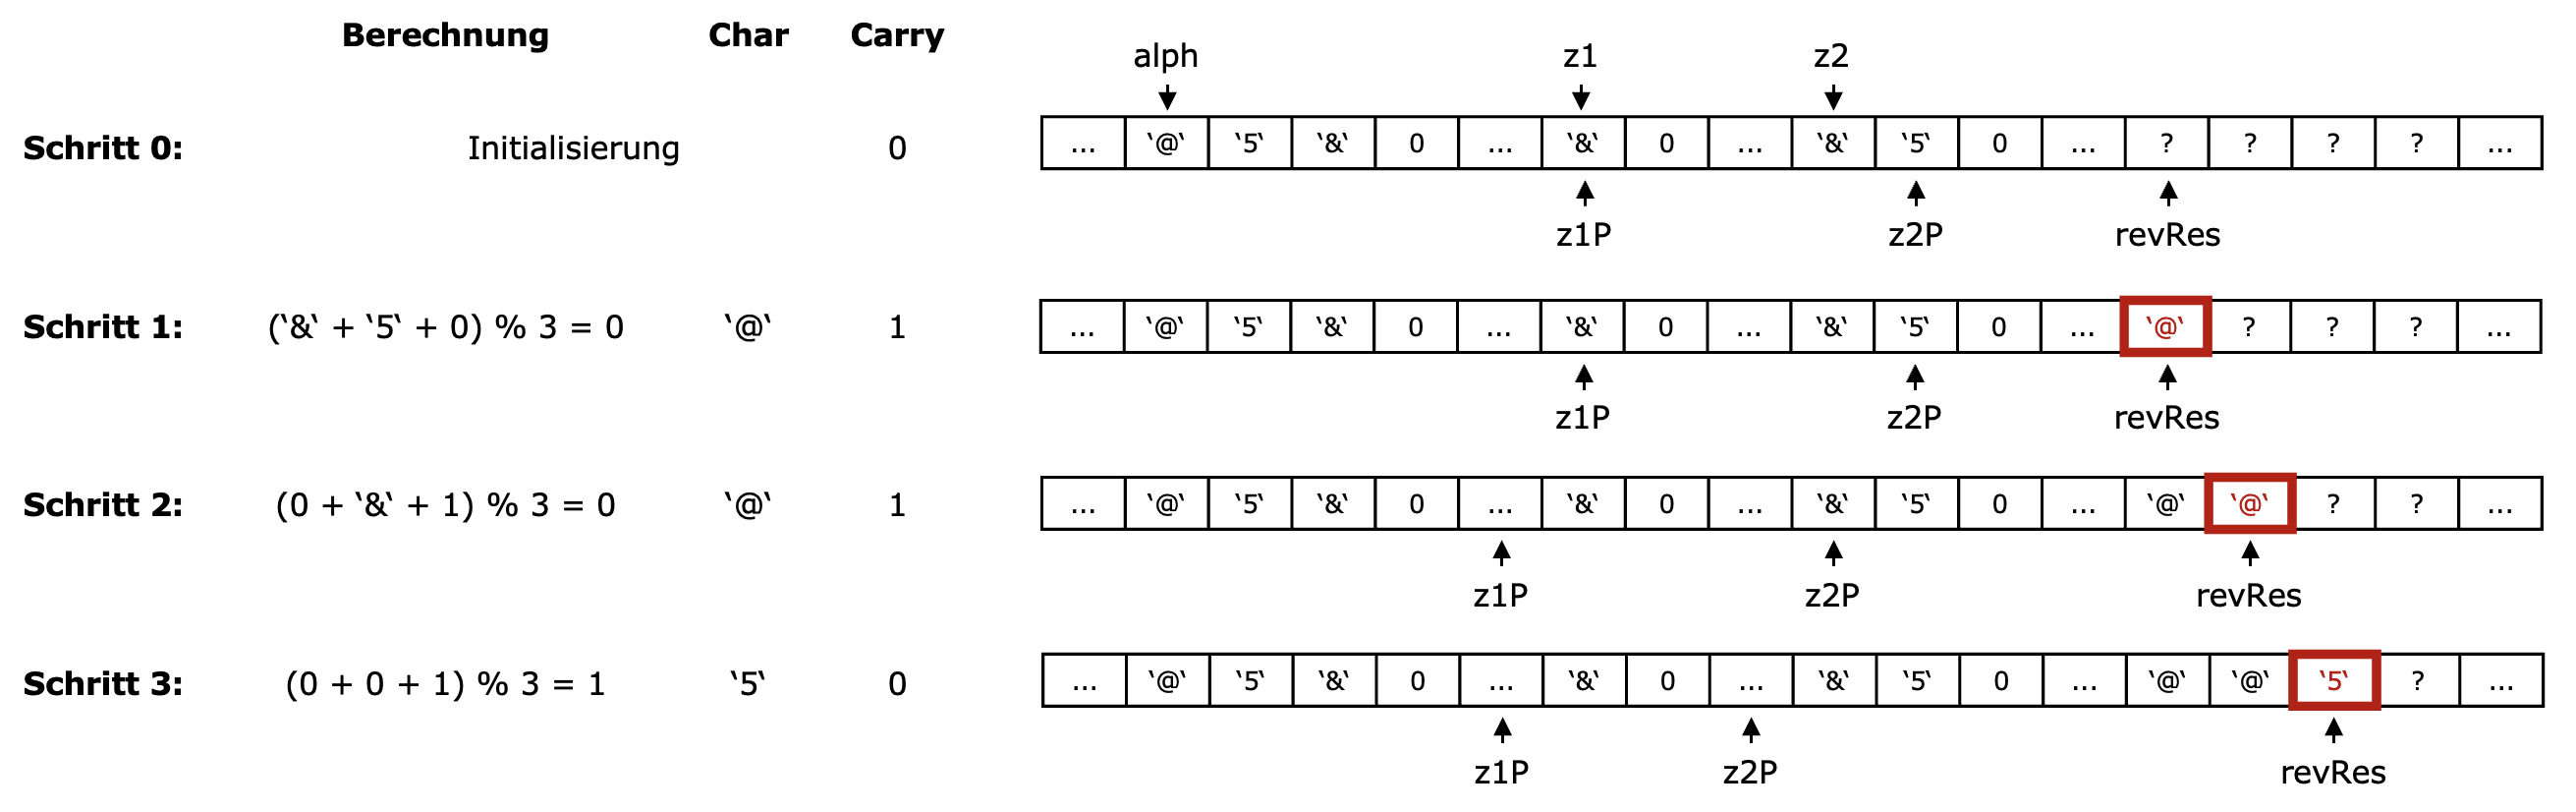
\includegraphics[width=\textwidth]{Abbildungen/ImplementierungAddition.png}
        \caption{Beispiel: Basis = 3, Alphabet = "@5\&", Operation: "\&" + "\&5" \ = "5@@"}\label{fig:ImplAdd}
    \end{figure}

    \verb+z1P+ und \verb+z2P+ laufen über die beiden Zahlen "\&" \ und "\&5", bis der erste Pointer (\verb+z1P+) vor den Anfang zeigt. Da
    dies nach Schritt 1 bei dem anderen Pointer (\verb+z2P+) noch nicht der Fall ist, geht der Vorgang weiter, jedoch wird der erste Summand
    automatisch auf 0 gesetzt. Nach Schritt 2 zeigt zwar auch \verb+z2P+ vor den Anfang des zweiten Operanden, der Übertrag ist aber ungleich
    0, weshalb Schritt 3 notwendig ist. Am Ende muss das Ergebnis aus \verb+revRes+ nur noch umgekehrt werden, wobei potenzielle,
    vorangestellte Nullen entfernt und ein '\verb+-+' an den Anfang gesetzt werden kann.\\
    \newline
    Schon in dem kleinen Beispiel aus Abbildung \ref{fig:ImplAdd} zeigt sich die Stärke der Implementierung. Dadurch, dass sich die Pointer
    \verb+z1P+ und \verb+z2P+ solange parallel verschieben, bis die kürzere Zahl abgearbeitet ist, der Pointer der längeren Zahl aber noch
    individuell dekrementiert wird, können die einzelnen Längen beliebig gewählt werden.\\
    \newline
    Bei der Multiplikation verläuft es anders, denn hier wird jede Stelle des einen Faktors nicht nur mit der gleichen Stelle des anderen
    Faktors multipliziert, sondern mit dem gesamten Faktor (siehe Abschnitt \ref{Multiplikation}). Daher laufen \verb+z1P+ und \verb+z2P+
    nicht parallel über die Zahlen, sondern bewegen sich wie folgt. \verb+z1P+ wird anfangs an der Einerstelle fixiert, während \verb+z2P+
    einmal von der Einer- bis zur höchsten Stelle durchläuft, und jeweils die Multiplikation der Stellen durchgeführt wird. Erst im nächsten
    Schritt wird \verb+z1P+ um eins erniedrigt, und \verb+z2P+ läuft erneut über die ganze Zahl. Dieser Vorgang wiederholt sich so lange, auch
    auch \verb+z1P+ die höchste Stelle erreicht, wobei die Zwischenergebnisse jeweils, mit der oben beschrieben Methode, addiert werden.
    Die Längen der Operanden können also auch hier komplett frei gewählt werden, da \verb+z1P+ und \verb+z2P+ unabhängig voneinander über
    die jeweiligen Strings iterieren.

    \subsection{Funktionsweise der Referenzimplementierung}\label{FunktRef}

    Um die Korrektheit und Performanz der Hauptimplementierung zu prüfen, wurde eine weitere Implementierung erstellt. Das Konzept sowie die
    Funktionalität sind dabei sehr ähnlich zu der Hauptimplementierung. Unterschiedlich ist, dass die Rechnungen nun nicht mehr im Zahlensystem
    der spezifizierten Basis stattfinden, sondern im Dezimalsystem. Nachdem die Operanden nämlich in dieses konvertiert wurden, können sämtliche
    Rechnungen vom Prozessor übernommen werden, und müssen nicht mehr manuell durchgeführt werden.\\
    \newline
    Ein praktisches Problem ergibt sich dabei allerdings hinsichtlich der Darstellbarkeit von Zahlen, die sich, zumindest in den
    Standard-Datentypen, auf eine bestimmte Größe begrenzt. Um Vergleiche zwischen Haupt- und Referenzimplementierung ziehen zu können, muss
    aber auch letztere mit Werten beliebiger Größe zurechtkommen, weshalb folgendermaßen Abhilfe geschaffen wird. Die Operanden werden, wie in
    der Implementierung oben, ebenfalls in Sub-Strings geteilt. Deren Länge umfasst jetzt aber nicht mehr nur einen \verb+char+, sondern so viele,
    dass sich der maximale Wert der konvertierten Zahl sowie das Ergebnis der jeweiligen Operation noch als \verb+int64_t+ darstellen lässt
    (\verb+maxLength+). Bei Addition und Subtraktion hat sich für diese Länge $\lfloor log_{basis}(2^{63} - 1)\rfloor $ als guter Wert herausgestellt, bei der
    Multiplikation $\lfloor log_{basis}(2^{63} - 1) / 2\rfloor $.\\
    \newline
    Dementsprechend werden für die Berechnungen zuerst Strings der Länge \verb+maxLength+ ins Dezimalsystem umgerechnet und anschließend miteinander
    verrechnet. Das Ergebnis wird wieder zurückkonvertiert und an den entsprechenden Speicherplatz gelegt. Am Ende jeder Iteration ändern sich
    die Pointer dann nicht nur um $\pm1$, sondern um \verb+maxLength+.

    \subsection{Exemplarische Tests beider Implementierungen}

    Um zu zeigen, dass die in diesem Kapitel vorgestellten Ansätze nicht nur konzeptionell richtig sind, sondern auch korrekt implementiert
    wurden, werden in diesem Abschnitt Ergebnisse exemplarischer Eingaben gezeigt (Tabelle \ref{tab:Tests}). Hierbei sei angemerkt, dass das
    Programm während der Entwicklung auch systematisch getestet wurde. Die entsprechenden Tests befinden sich im Order
    \verb+Implementierung/Tests+, und können durch \verb+make all+  und \verb+./add+, \verb+./sub+, \verb+./mul+ (alle für Hauptimplementierung)
    oder \verb+./conv+ (Referenz) ausgeführt werden.

    \begin{table}[h]
        \centering
        \begin{tabular}{cc}
            \toprule
            \textit{Test 1} & 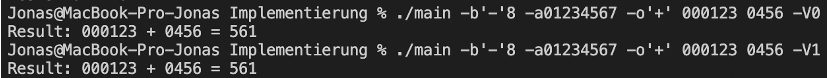
\includegraphics[width=12cm]{Abbildungen/Eingabe1.png} \\
            \textit{Test 2} & 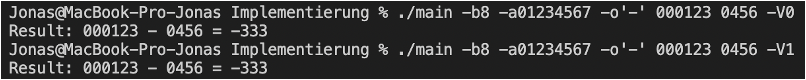
\includegraphics[width=12cm]{Abbildungen/Eingabe2.png} \\
            \textit{Test 3} & 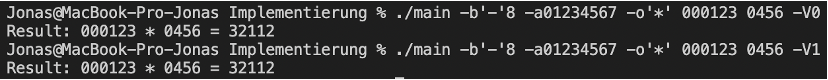
\includegraphics[width=12cm]{Abbildungen/Eingabe3.png} \\
            \textit{Test 4} & 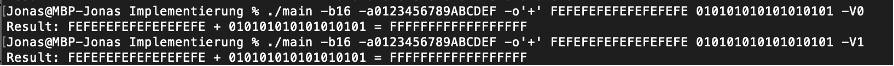
\includegraphics[width=12cm]{Abbildungen/Eingabe4.png} \\
            \textit{Test 5} & 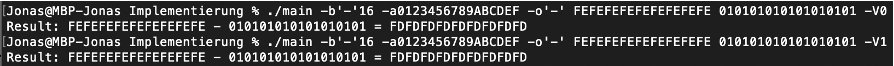
\includegraphics[width=12cm]{Abbildungen/Eingabe5.png} \\
            \textit{Test 6} & 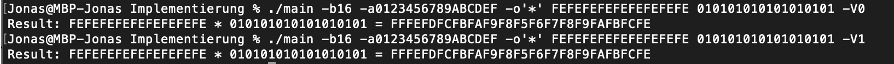
\includegraphics[width=12cm]{Abbildungen/Eingabe6.png} \\
            \bottomrule
        \end{tabular}
        \caption{Beispielhafte Ein- und Ausgaben des Programms, jeweils für Haupt- (-V0) und Referenzimplementierung (-V1)}\label{tab:Tests}
    \end{table}

    Die ersten drei Tests zeigen exemplarisch, dass alle drei Operationen jeweils bei kleinen Instanzen funktionieren. Dass die Werte in
    \textit{Test 1} und \textit{Test 3} dabei auf der $-8$, die in \textit{Test 2} hingegen auf der $8$ basieren, belegt außerdem, dass in
    Zahlensystemen mit sowohl positiven als auch mit negativen Basen einwandfrei gerechnet werden kann. Bezüglich der Referenzimplementierung
    ist zudem interessant, dass das Konvertieren von Systemen mit Basis ungleich zehn problemlos in beide Richtungen konvertiert werden
    können. Weiter ist auffällig, dass zwar bei allen Operanden vorangestellte Nullen zu sehen sind, diese aber keinerlei Auswirkungen auf die
    Ergebnisse haben.\\
    \newline
    Zu Beginn des Kapitels wird erwähnt, dass das Programm nicht nur Rechnungen mit Werten diverser Basen anstellen können muss, sondern dass
    diese Werte auch beliebig lange sein können sollen. Dass beide Implementierungen auch dieses Feature anbieten,
    soll mithilfe der nächsten drei Tests gezeigt werden. Dafür wurden jeweils zwei Operanden ausgesucht, die mit einer Länge von 18
    beziehungsweise 17 Bytes sogar den Darstellungsbereich des Typs \verb+int128_t+ überschreiten. Dennoch wird ohne Probleme von beiden
    Implementierungen immer das richtige Ergebnis ausgegeben. Dies zeigt auch, dass die in Abschnitt \ref{FunktRef} gezeigten Formeln für die
    \verb+maxLength+ richtig sind.


    \section{Performanzanalyse}

    Bevor die eigentliche Performanz unseres Programmes analysiert werden kann, müssen wir zuerst die Messbedingungen klären. Die Messungen wurden
    auf einem Macbook Air M1 bei der Compiler-Stufe O3 durchgeführt. Außerdem wurden für jeden Messpunkt 15 unterschiedliche String-Paare
    zufällig generiert und jedes Paar 15-mal verrechnet. Um möglichst präzise Ergebnisse unseres Programms zu bekommen, wurde die Durchschnitte
    aller Laufzeiten genommen und berechnet. Das Intervall, in dem die Werte gemessen wurden, fängt bei 50 Zeichen an
    und endet bei 2000 Zeichen. Alle generierten Zahlen sind dabei Zahlen der Basis 50. \\

    \subsection{Performanz der Addition und Subtraktion}

    Zuerst betrachten wir die Performanz der Addition und der Subtraktion. Die folgenden beiden Abbildungen
    zeigen die Resultate beider Implementationen, wobei $V0$ unsere Hauptimplementierung darstellt und $V1$ unsere
    Referenzimplementierung. \\


    \begin{figure}[ht]
        \captionsetup{justification=centering}
        \begin{tikzpicture}
            \pgfplotsset{every axis legend/.append style={
                at={(0.5,1.03)},
                anchor=south}}
            \begin{axis}
            [legend columns=2,width=3in,name=additiong, xlabel={Länge der Eingabe},ylabel={Gesamtzeit in Mikrosekunden},
                ymin=0,ymax=40,xmin=0,xmax=2000]


                \addplot[blue,mark=o] table{data/addition.txt};
                \addplot[red,mark=x] table{data/V1Addition.txt};



                \legend{$V0$,$V1$}
            \end{axis}
            \node[anchor=north] at (additiong.north) { Addition};


        \end{tikzpicture}
        \begin{tikzpicture}

            \pgfplotsset{every axis legend/.append style={
                at={(0.5,1.03)},
                anchor=south}}
            \begin{axis}
            [legend columns=2,width=3in,name=subtractiong, xlabel={Länge der Eingabe},
                ylabel={Gesamtzeit in Mikrosekunden},
                ymin=0,ymax=40,xmin=0,xmax=2000]
                \addplot[blue,mark=o] table{data/subtraction.txt};
                \addplot[red,mark=x] table{data/V1Subtraction.txt};

                \legend{$V0$,$V1$}
            \end{axis}
            \node[anchor=north] at (subtractiong.north) { Subtraktion};

        \end{tikzpicture}
        \caption{Performanz der Addition und der Subtraktion beider Implementierungen}
    \end{figure}

    Was bei beiden Funktionalitäten und beiden Implementierungen positiv auffällt, ist die Tatsache,
    dass beide Algorithmen in linearer Zeit laufen. Jedoch ist unsere Referenzimplementierung im Gegensatz zu der
    Hauptimplementierung ca. um den Faktor $0.5$ langsamer. Somit können wir allgemein sagen, dass unsere Hauptimplementierung,
    auch wenn die Referenzimplementierung trotzdem gute Ergebnisse liefert, trotzdem bei der Addition bzw. Subtraktion bevorzugt werden
    sollte.

    \subsection{Performanz der Multiplikation}

    Die Multiplikation ist natürlich auch ein wichtiger Bestandteil beider Implementierungen. Die zwei folgenden Abbildungen stellen dabei einmal
    die Performanz der beiden Implementierungen gegenüber (linke Abbildung) und auch deren Wachstumsraten (rechte Abbildung). \\

    \begin{figure}[ht]
        \captionsetup{justification=centering}
        \begin{tikzpicture}
            \pgfplotsset{every axis legend/.append style={
                at={(0.5,1.03)},
                anchor=south}}
            \begin{axis}
            [legend columns=2,name=multiplicationg,width=3in, xlabel={Länge der Eingabe},ylabel={Gesamtzeit in Mikrosekunden},
                ymin=0,ymax=60000,xmin=0,xmax=2000]
                \addplot[blue,mark=o] table{data/multiplication.txt};
                \addplot[red,mark=x] table{data/V1Multiplication.txt};
                \legend{$V0$,$V1$}
            \end{axis}
            \node[anchor=north] at (multiplicationg.north) {Multiplikation};
        \end{tikzpicture}
        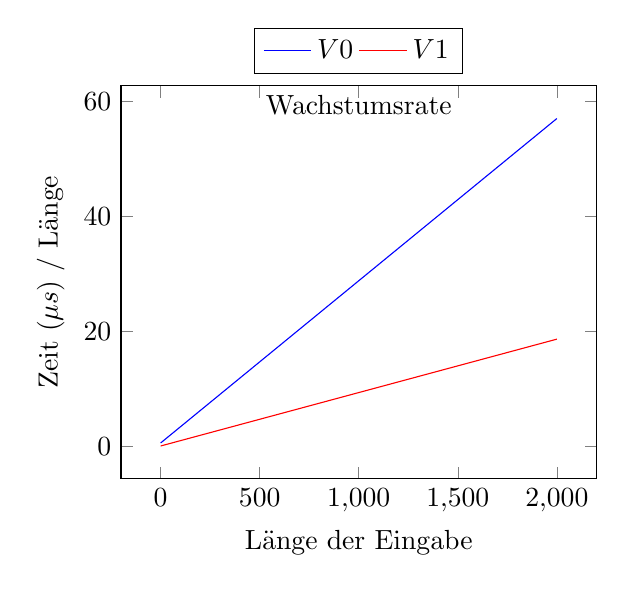
\begin{tikzpicture}
            \pgfplotsset{every axis legend/.append style={
                at={(0.5,1.03)},
                anchor=south}}
            \begin{axis}
                [legend columns=2,name=slopeg,width=3in,
                domain=0.125:2000,xlabel={Länge der Eingabe},ylabel={ Zeit ($\mu s$) / Länge  }]

                \addplot[ blue]  { 0.02822*x + 0.6264};
                \addplot[ red]  {0.0092928*x + 0.1054};


                \legend{$V0$,$V1$}
            \end{axis}
            \node[anchor=north] at (slopeg.north) { Wachstumsrate};
        \end{tikzpicture}
        \caption{Performanz der Multiplikation beider Implementierungen und deren Wachstumsraten}
    \end{figure}

    Die erste Erkenntnis, die man aus der linken Abbildung entnehmen kann, ist, dass beide Implementierungen
    sich in quadratischen Laufzeitklassen befinden. Auch wenn das für die Multiplikation nicht verwunderlich, da dabei ja immer eine Zahl
    mit allen anderen Ziffern der anderen Zahl multipliziert werden, ist vor allem die Wachstumsrate der Hauptimplementierung sehr bedenklich,
    da diese mit einem Faktor von ca. $3$ schneller wächst, als die Referenzimplementierung, was vor allem bei größeren Eingabelängen
    die Laufzeit fast schon exponentiell wachsen lässt.

    \subsection{Bewertung der Performanzanalyse}

    Somit kann kurz zusammengefasst werden, das beide Implementierungen gute Resultate liefern, es jedoch nicht so ist,
    dass eine Implementierung bedeutend schneller als die andere läuft. Falls einem die Performanz bei der Addition bzw. Subtraktion wichtig ist,
    so sollte man in den meisten Fällen auf die Hauptimplementierung zurückgreifen. Wenn man aber eine performante Multiplikation haben möchte, bietet sich
    die Referenzimplementierung eher an. \\


    \section{Zusammenfassung und Ausblick}

    Die Aufgabenstellung hat nach einer Umsetzung der Ausführung arithmetischer Operationen auf
    g-adischen Zahlen verlangt, die in ihrer Länge nicht limitiert seien dürfen. Diese Aufgabe wurde auf zwei
    verschiedene Arten und Weisen realisiert. Einmal durch das direkte Verrechnen der Zahlen ohne Konvertierung und
    einmal durch eine Hybrid-Implementierung, welche die Zahlen teilweise konvertiert und danach die Zwischenergebnisse gemäß der
    gegebenen arithmetischen Operation miteinander verrechnet. Dabei erzielten beide Lösungsansätze für bestimmte Operation bessere bzw. schlechtere
    Performanz im Gegensatz zu der anderen Implementierung. Somit können wir abschließend sagen, dass beide Implementierungen ihre Daseinsberechtigung haben
    und man potenziell in einer tatsächlichen Veröffentlichung auch beide Ansätze zusammenführen könnte, um so immer die beste Performanz für den Endnutzer
    zu erzielen.

% TODO: Fuegen Sie Ihre Quellen der Datei Ausarbeitung.bib hinzu
% Referenzieren Sie diese dann mit \cite{}.
% Beispiel: CR2 ist ein Register der x86-Architektur~\cite{intel2017man}.
    \bibliographystyle{plain}
    \bibliography{Ausarbeitung}{}

\end{document}
